\documentclass[12pt, a4paper, oneside]{ctexart}
\usepackage{amsmath, amsthm, amssymb, bm, color, graphicx, geometry, hyperref, mathrsfs,extarrows, braket, booktabs, array, diagbox}

\linespread{1.5}
%\geometry{left=2.54cm,right=2.54cm,top=3.18cm,bottom=3.18cm}
\geometry{left=1.84cm,right=1.84cm,top=2.18cm,bottom=2.18cm}
\newenvironment{problem}{\par\noindent\textbf{题目. }}{\bigskip\par}
\newenvironment{solution}{\par\noindent\textbf{解答. }}{\bigskip\par}
\newenvironment{note}{\par\noindent\textbf{注记. }}{\bigskip\par}

% 基本信息
\newcommand{\RQ}{\today} % 日期
\newcommand{\km}{概率论} % 科目
\newcommand{\bj}{强基数学002} % 班级
\newcommand{\xm}{吴天阳} % 姓名
\newcommand{\xh}{2204210460} % 学号

\begin{document}

%\pagestyle{empty}
\pagestyle{plain}
\vspace*{-15ex}
\centerline{\begin{tabular}{*5{c}}
    \parbox[t]{0.25\linewidth}{\begin{center}\textbf{日期}\\ \large \textcolor{blue}{\RQ}\end{center}} 
    & \parbox[t]{0.2\linewidth}{\begin{center}\textbf{科目}\\ \large \textcolor{blue}{\km}\end{center}}
    & \parbox[t]{0.2\linewidth}{\begin{center}\textbf{班级}\\ \large \textcolor{blue}{\bj}\end{center}}
    & \parbox[t]{0.1\linewidth}{\begin{center}\textbf{姓名}\\ \large \textcolor{blue}{\xm}\end{center}}
    & \parbox[t]{0.15\linewidth}{\begin{center}\textbf{学号}\\ \large \textcolor{blue}{\xh}\end{center}} \\ \hline
\end{tabular}}
\vspace*{4ex}

% 正文部分
\paragraph{习题 4.1}
\paragraph{2.}甲从$1,2,3,4$中任取一数$X$,乙再从$1,\cdots,X$中任取一数$Y$。试求$(X,Y)$的联合分布。
\renewcommand\arraystretch{0.8} % 设置表格高度为原来的0.8倍
\begin{table}[!htbp] % table标准
    \centering % 表格居中
    \begin{tabular}{p{3cm}<{\centering}|p{3cm}<{\centering}p{3cm}<{\centering}p{3cm}<{\centering}p{3cm}<{\centering}} % 设置表格宽度
    %\begin{tabular}{cccc}
        \toprule
        \diagbox{X}{Y} & $1$ & $2$ & $3$ & $4$ \\
        \midrule
        $1$ & $1/4$ & $0$ & $0$ & $0$ \\ 
        $2$ & $1/8$ & $1/8$ & $0$ & $0$ \\ 
        $3$ & $1/12$ & $1/12$ & $1/12$ & $0$ \\ 
        $3$ & $1/16$ & $1/16$ & $1/16$ & $1/16$ \\ 
        \bottomrule
    \end{tabular}
\end{table}

\paragraph{4.}试问:函数
\begin{equation*}
    p(x_1,x_2,x_3)=x_1^2+6x_3^2+\frac{x_1x_2}{3},\quad 0 < x_1 < 1,\ 0 < x_2<2, 0 < x_3 < \frac{1}{2}
\end{equation*}
是否为一随机向量的密度函数?
\begin{solution}
    由于
    \begin{equation*}
        \begin{aligned}
            \int_0^1\int_0^2\int_0^{1/2}\left(x_1^2+6x_3^2+\frac{x_1x_2}{3}\right)\,dx_3\,dx_2\,dx_1 =&\  
            \int_0^1x_1^2\,dx_1+12\int_0^{1/2}x_3^2\,dx_3+\frac{1}{6}\int_0^1\int_0^2x_1x_2\,dx_2\,dx_1\\
            =&\ \frac{1}{3} + \frac{1}{2} + \frac{1}{6} = 1
        \end{aligned}
    \end{equation*}
    所以$p(x_1,x_2,x_3)$是一随机向量的密度函数。
\end{solution}
\def\P{\mathbf{P}}
\def\disp{\displaystyle}
\paragraph{6.}设随机向量$(X, Y)$的密度函数为
\begin{equation*}
    p(x, y) = ce^{-(3x+4y)},\quad x > 0,\ y > 0.
\end{equation*}
试求:(1) 常数$c$;(2) 联合分布函数$F(x, y)$;(3) $\P\{0<X\leqslant 1,\ 0< Y \leqslant 2\}$。
\begin{solution}
    (1)\begin{equation*}
        \int_0^{+\infty}\int_0^{+\infty}ce^{-(3x+4y)}\,dy\,dx = c\int_0^{+\infty}\frac{1}{4}e^{-3x}\,dx = \frac{c}{12} = 1
    \end{equation*}
    所以$ c = 12$。

    (2) $\disp F(x, y) = \int_0^x\int_0^y12e^{-(3u+4v)\,dv\,du} = \int_0^x-3e^{-3u}(e^{-4y}-1)\,du = (e^{-3x}-1)(e^{-4y}-1)$

    (3) $\disp \P\{0<X\leqslant 1,\ 0< Y \leqslant 2\} = F(1, 2) - F(0, 2)- F(1, 0)+ F(0,0) = (e^{-3}-1)(e^{-8}-1)$
\end{solution}
\paragraph{8.}设$(X,Y)$的联合密度函数为
\begin{equation*}
    p(x, y) = cxy^2,\quad 0 < x <  2,\quad 0 < y < 1.
\end{equation*}
试求:$(1)$ 常数$c$;(2) $X, Y$至少有一个小于$\disp\frac{1}{2}$的概率。
\begin{solution}
    (1) $\disp \int_0^2cxy^2\,dy\,dx = \int_0^2\frac{c}{3}x\,dx = \frac{2}{3}c = 1$,则$\disp c = \frac{3}{2}$。

    (2) 由于$\disp p(x, y) = \frac{3}{2}xy^2$,则
    \begin{equation*}
        \begin{aligned}
            \P((X < \frac{1}{2})\cup (Y < \frac{1}{2})) =&\ 1-\P((X\geqslant \frac{1}{2})\cap(Y\geqslant \frac{1}{2}))\\
             =&\ 1-\int_{1/2}^2\int_{1/2}^1\frac{3}{2}xy^2\,dy\,dx = 1-\frac{7}{16}\int_{1/2}^2x\,dx = \frac{23}{128}
        \end{aligned}
    \end{equation*}
\end{solution}
\paragraph{习题 4.2}
\paragraph{1.}证明多项分布的边缘分布仍为多项分布.
\begin{proof}
    设$(X_1,X_2,\cdots,X_n)\sim M_n(m; p_1,p_2,\cdots,p_n)$,对于任意的$k = 1,2,\cdots, n-1$,有
    \begin{equation*}
        \begin{aligned}
            &\ \P(X_1=m_1,X_2=m_2,\cdots,X_k=m_k)\\
            =&\ \sum_{m_{k+1}+\cdots+m_n=m-m_1-\cdots-m_k}\P(X_1 = m_1,X_2=m_2,\cdots,X_k = m_k)\\
            =&\ \sum_{m_{k+1}+\cdots+m_n=m-m_1-\cdots-m_k}\frac{m!}{m_1!\cdots m_n!}p_1^{m_1}\cdots p_n^{m_n}\\
            =&\ \frac{m!\cdot p_1^{m_1}\cdots p_k^{m_k}}{m_1!\cdots m_k!(m-m_1-\cdots-m_k)!}\sum_{m_{k+1}+\cdots+m_n=m-m_1-\cdots-m_k}\frac{(m-m_1-\cdots-m_k)!}{m_{k+1}!\cdots m_n!}p_{k+1}^{m_{k+1}}\cdots p_n^{m_n}\\
            =&\ \frac{m!}{m_1!\cdots m_k!(m-m_1-\cdots-m_k)!}p_1^{m_1}\cdots p_k^{m_k}(p_{k+1}+\cdots+p_n)^{m-m_1-\cdots-m_k}\\
            =&\ \frac{m!}{m_1!\cdots m_k!(m-m_1-\cdots-m_k)!}p_1^{m_1}\cdots p_k^{m_k}(1-p_1-\cdots-p_k)^{m-m_1-\cdots-m_k}\\
        \end{aligned}
    \end{equation*}
    则$(X_1,X_2,\cdots,X_k)$的边缘分布为$M_{k+1}(m;p_1,p_2,\cdots,p_k,1-p_1-p_2-\cdots-p_k)$.
    
    同理可证,对于任意的指标集$\{i_1,i_2,\cdots,i_k\}\ (1\leqslant i_j\leqslant n)$,有$(X_{i_1},X_{i_2},\cdots,X_{i_k})$的边缘分布为$M_{k+1}(m;p_1,p_2,\cdots,p_k,1-p_1-p_2-\cdots-p_k)$.所以, 多项分布的边缘分布仍为多项分布.
\end{proof}
\paragraph{3.}设随机向量$(X,Y)$的联合密度为\begin{equation*}
    p(x, y) = \frac{1}{\Gamma(k_1)\Gamma(k_2)}x^{k_1-1}(y-x)^{k_2-1}e^{-y},
\end{equation*}
其中$k_1>0,\ k_2 > 0,\ 0 < x\leqslant y < \infty$. 试求$X$与$Y$的边缘分布密度.
\begin{solution}
    \begin{equation*}
        \begin{aligned}
            p_1(x) = \int_{-\infty}^{\infty}p(x, v)\,dv =&\ \frac{x^{k_1-1}}{\Gamma(k_1)\Gamma(k_2)}\int_x^{\infty}(v-x)^{k_2-1}e^{-v}\,dv\\
            \xlongequal{t = v-x}&\ \frac{x^{k_1-1}e^{-x}}{\Gamma(k_1)\Gamma(k_2)}\int_0^{\infty}t^{k_2-1}e^{-t}\,dt\\
            =&\ \frac{x^{k_1-1}e^{-x}}{\Gamma(k_1)\Gamma(k_2)}\Gamma(k_2) = \frac{x^{k_1-1}e^{-x}}{\Gamma(k_1)}\\
            p_2(y) = \int_{-\infty}^{\infty}p(u, y)\,du =&\ \frac{e^{-y}}{\Gamma(k_1)\Gamma(k_2)}\int_0^yu^{k_1-1}(y-u)^{k_2-1}\,du\\
            \xlongequal{t = u/y}&\ \frac{e^{-y}}{\Gamma(k_1)\Gamma(k_2)}\int_0^1(yt)^{k_1-1}(y-yt)^{k_2-1}y\,dt\\
            =&\ \frac{y^{k_1+k_2-1}e^{-y}}{\Gamma(k_1)\Gamma(k_2)}\int_0^1t^{k_1-1}(1-t)^{k_2-1}\,dt\\
            =&\ \frac{y^{k_1+k_2-1}e^{-y}}{\Gamma(k_1)\Gamma(k_2)}B(k_1,k_2)\\
            =&\ \frac{y^{k_1+k_2-1}e^{-y}}{\Gamma(k_1)\Gamma(k_2)}\,\frac{\Gamma(k_1)\Gamma(k_2)}{\Gamma(k_1+k_2)}\\
            =&\ \frac{y^{k_1+k_2-1}e^{-y}}{\Gamma(k_1+k_2)}\\
        \end{aligned}
    \end{equation*}
\end{solution}
\paragraph{5.}设$F(x, y)$和$G(x,y)$分别是二维随机向量$(X_1,Y_1)$和$(X_2,Y_2)$的联合分布函数. 记\begin{equation*}
    \bar{F}(x, y) = \P(X_1 > x,\ Y_1 > y),\quad \bar{G}(x, y)=\P(X_2 > x,\ Y_2 > y).
\end{equation*}
若$(X_1,Y_1)$和$(X_2,Y_2)$具有相同的边缘分布, 这证明$F(x, y)\leqslant G(x, y)$当且仅当$\bar{F}(x, y)\leqslant \bar{G}(x, y).$
\begin{proof}
    由题可知, 边缘分布$\disp \bar{F}_1(x) = \P(X_1 > x) = 1-\P(X\leqslant x) = 1-G(X\leqslant x) = \bar{G}_1(x)$, 同理可得, $\bar{F}_2(y) = \bar{G}_2(y)$. 又由于
    \begin{equation*}
        \begin{aligned}
        F(x, y) =&\ 1 - (\bar{F}_1(x)+\bar{F}_2(y) - \bar{F}(x, y)) = \bar{F}(x, y) + 1 - \bar{F}_1(x) - \bar{F}_2(y)\\
        G(x, y) =&\ 1 - (\bar{G}_1(x)+\bar{G}_2(y) - \bar{G}(x, y)) = \bar{G}(x, y) + 1 - \bar{G}_1(x) - \bar{G}_2(y)
        \end{aligned}
    \end{equation*}
    则\begin{equation*}
        \begin{aligned}
            F(x, y)\leqslant G(x, y)\iff&\ \bar{F}(x, y) + 1 - \bar{F}_1(x) - \bar{F}_2(y)\leqslant \bar{G}(x, y) + 1 - \bar{G}_1(x) - \bar{G}_2(y)\\
            \iff&\ \bar{F}(x, y)\leqslant \bar{G}(x, y)
        \end{aligned}
    \end{equation*}
\end{proof}
\paragraph{6.}设随机变量$(X,Y)$的联合密度函数为
\begin{equation*}
    p(x, y) = \frac{1+xy}{4},\quad |x| < 1\ \text{且}\ |y| < 1.
\end{equation*}
证明: $X$与$Y$不独立, 但$X^2$与$Y^2$是独立的.
\begin{proof}
    $X$的边缘密度为$\disp p_1(x) = \int_{-1}^{1}\frac{1+xv}{4}\,dv = \frac{1}{2}$, 由轮换对称性可知, $\disp p_2(y) = \frac{1}{2}$, 则$X$的边缘分布为$\disp F_1(x) = \int_{-1}^xp_1(u)\,du = \frac{x+1}{2}$, 同理$\disp F_2(y) = \frac{y+1}{2}$, 于是$\disp F_1(x)F_2(y) = \frac{(x+1)(y+1)}{4}$, 而
    \begin{equation*}
        F(x, y) = \P(X\leqslant x,\ Y\leqslant y) = \int_{-1}^x\int_{-1}^y\frac{1+uv}{4}\,du\,dv = \frac{1}{4}(x+1)(y+1)((x-1)(y-1)+1)
    \end{equation*}
    所以$F_1(x)F_2(y)\neq F(x, y)$, 于是$X$与$Y$不独立.

    $X^2$的概率分布为$F_1'(x) = \P(X^2\leqslant x) = F_1(\sqrt{x}) - F_1(-\sqrt{x}) = \sqrt{x}$, 同理, $Y^2$的概率分布为$F_2'(y) = \sqrt{y}$, 由于
    \begin{equation*}
        F'(x, y) = \P(X^2\leqslant x,\ Y^2\leqslant y) = \int_{-\sqrt{x}}^{\sqrt{x}}\int_{-\sqrt{y}}^{\sqrt{y}}\frac{1+uv}{4}\,du\,dv = \sqrt{xy}
    \end{equation*}
    所以$F_1'(x)F_2'(y) = F'(x, y)$, 于是$X^2$与$Y^2$是独立的.
\end{proof}
\paragraph{7.}若$X,Y$独立, 都服从$-1$与$1$这两点上的等可能分布, 而$Z = XY$. 证明:$X,Y,Z$两两独立但不相互独立.
\begin{proof}不难验证$Z$与$X,Y$服从相同的分布律, 于是
    \begin{equation*}
        \begin{aligned}
            F(X\leqslant -1, Z\leqslant -1) =&\  F(X=-1,Y=1) = \frac{1}{4} = F(X\leqslant -1)F(Z\leqslant -1)\\
            F(X\leqslant -1, Z\leqslant 1) =&\  F(X=-1,Y=\pm 1) = \frac{1}{2} = F(X\leqslant -1)F(Z\leqslant 1)\\
            F(X\leqslant 1, Z\leqslant -1) =&\  \P(X=-1,Y= 1)+\P(X=1, Y=-1) = \frac{1}{2} = F(X\leqslant 1)F(Z\leqslant -1)\\
            F(X\leqslant 1, Z\leqslant 1) =&\  \P(X=1,Y= 1) = 1 = F(X\leqslant 1)F(Z\leqslant 1)\\
        \end{aligned}
    \end{equation*}
    所以$X,Z$独立, 同理可得, $Y,Z$独立, 于是$X,Y,Z$两两独立. 由于
    \begin{equation*}
        F(X\leqslant -1,\ Y\leqslant -1,\ Z\leqslant -1) = 0 \neq F(X\leqslant -1)F(Y\leqslant -1)F(Z\leqslant -1) = \frac{1}{8}
    \end{equation*}
    所以$X,Y,Z$不相互独立.
\end{proof}
\paragraph{习题 4.3}
\paragraph{1.}设随机向量$(X,Y,Z)$服从单位球$\disp D = \left\{(x, y, z):x^2+y^2+z^2 < 1\right\}$上的均匀分布, (1) 试求$X$的边缘分布; (2) 试求$X$在给定$Y,Z$的条件密度函数.
\begin{solution}
    (1) $x$的边缘密度为
    \begin{equation*}
        \begin{aligned}
            p_1(x) = \int_{y^2+z^2 < 1-x^2}\frac{3}{4\pi}\, dy\,dz = \int_0^{\sqrt{1-x^2}}\int_0^{2\pi}\frac{3}{4\pi}r\,d\theta\,dr=\frac{3}{4}(1-x^2)
        \end{aligned}
    \end{equation*}
    则$X$的边缘分布为
    \begin{equation*}
        F(x) = \int_{-1}^x\frac{3}{4}(1-u^2)\,du = \frac{1}{4}(-x^3+3x+2)
    \end{equation*}

    (2) 给定$y,z$的边缘密度函数为$\disp p_2(y, z) = \int_{-\sqrt{1-y^2-z^2}}^{\sqrt{1-y^2-z^2}}\frac{3}{4\pi}\,dx = \frac{3}{2\pi}\sqrt{1-y^2-z^2}$, 则条件密度函数为
    \begin{equation*}
        p_3(x|y, z) = \frac{p(x, y, z)}{p_2(y, z)} = \frac{1}{2\sqrt{1-y^2-z^2}}
    \end{equation*}
\end{solution}
\paragraph{3.}若$(X,Y)$服从二维正态分布$\mathcal{N}(a, b;\sigma_1^2,\sigma_2^2; r)$, 以$D(\lambda)$记下面椭圆的内部
\begin{equation*}
    \frac{(x-a)^2}{\sigma_1^2}-\frac{2r(x-a)(y-b)}{\sigma_1\sigma_2}+\frac{(y-b)^2}{\sigma_2^2} = \lambda^2,
\end{equation*}
试求概率$\P\{(X,Y)\in D(\lambda)\}$.
\begin{solution}
    做变换$\varphi(x, y) = (\sigma_1 u + a, \sigma_2 v + b)$, 则$|\varphi'(x, y)| = \sigma_1\sigma_2$, 记$\Omega$为$D(\lambda)$所围成的区域, 于是
    \begin{equation*}
        \begin{aligned}
            \P\{(X, Y)\in D(\lambda)\} =&\ \int_{\Omega}\frac{1}{2\pi\sigma_1\sigma_2\sqrt{1-r^2}}\exp\left\{-\frac{\lambda^2}{2(1-r^2)}\right\}\,dx\,dy\\
            \xlongequal{\varphi}&\ \int_{\varphi(\Omega)}\frac{1}{2\pi\sigma_1\sigma_2\sqrt{1-r^2}}\exp\left\{-\frac{\lambda^2}{2(1-r^2)}\right\}\sigma_1\sigma_2\,du\,dv\\
            =&\ \frac{1}{2\pi\sigma_1\sigma_2\sqrt{1-r^2}}\exp\left\{-\frac{\lambda^2}{2(1-r^2)}\right\}\int_{\varphi(\Omega)}\,du\,dv\\
            =&\ \frac{1}{2\pi\sigma_1\sigma_2\sqrt{1-r^2}}\exp\left\{-\frac{\lambda^2}{2(1-r^2)}\right\}S(\sigma(\Omega))\\
        \end{aligned}
    \end{equation*}
    由于$\sigma(\Omega)$是椭圆$u^2-2ruv+v^2 = \lambda^2$所围成的区域, 做旋转变换$\psi$:
    \begin{equation*}
        \psi\left(\left[\begin{matrix}
            u\\v
        \end{matrix}\right]\right) = \left[\begin{matrix}
            \cos\frac{\pi}{4}&\sin\frac{\pi}{4}\\
            -\sin\frac{\pi}{4}&\cos\frac{\pi}{4}\\
        \end{matrix}\right]\left[\begin{matrix}
            x\\y
        \end{matrix}\right] = \left[\begin{matrix}
            x+y\\-x+y
        \end{matrix}\right]
    \end{equation*}
    于是$S(\sigma(\Omega)) = S(\psi(\sigma(\Omega)))$, 是椭圆$\disp \frac{x^2}{\frac{\lambda^2}{2(1+r)}}+\frac{y^2}{\frac{\lambda^2}{2(1-r)}} = 1$所围成的面积, 所以$\disp S(\psi(\sigma(\Omega))) = \pi \sqrt{\frac{\lambda^2}{2(1+r)}\frac{\lambda^2}{2(1-r)}} = \pi\frac{\lambda^2}{2\sqrt{1-r^2}}$, 综上
    \begin{equation*}
        \P\{(X, Y)\in D(\lambda)\} = \frac{1}{2\pi\sqrt{1-r^2}}\exp\left\{-\frac{\lambda^2}{2(1-r^2)}\right\}\frac{\pi\lambda^2}{2\sqrt{1-r^2}} = \frac{\lambda^2}{4(1-r^2)}\exp\left\{-\frac{\lambda^2}{2(1-r^2)}\right\}
    \end{equation*}
\end{solution}
\paragraph{习题 4.4}
\paragraph{1.}设$X,Y$为相互独立的均服从区间$[0,1]$上均匀分布的随机变量, 试求$Z = X+Y$的分布函数密度.
\begin{solution}
    设$p(x, y)$为$X,Y$的联合密度函数, 则$p(x, y) = p(x)p(y) = 1,\ 0\leqslant x, y\leqslant 1$, 所以
    \begin{equation*}
        \begin{aligned}
            p_{Z}(x) = \int_{-\infty}^{\infty}p_X(x-t)p_Y(t)\,dt =&\  
            \begin{cases}
                \disp\int_0^xp(x-t,t)\,dt,&\quad 0\leqslant x\leqslant 1,\\
                \disp\int_{x-1}^1p(x-t,t)\,dt,&\quad 1 < x \leqslant 2.
            \end{cases}\\
            \Rightarrow \quad p_Z(x)=&\ \begin{cases}
                x,&\quad 0\leqslant x\leqslant 1,\\
                2-x, &\quad 1 < x\leqslant 2.
            \end{cases}
        \end{aligned}
    \end{equation*}
\end{solution}
\paragraph{2.}设随机变量$X,Y$相互独立, 密度函数均为$p(x) = e^{-x},\ x > 0$, 试问: $X+Y$与$\dfrac{X}{X+Y}$是否相互独立?
\begin{solution}
    设$p(x, y)$为$X,Y$的联合密度函数, 则$\disp p(x, y) = e^{-x-y},\ x, y > 0$, 则
    \begin{equation*}
        p_{X+Y}(x)  = \int_0^xp(x-t,t)\,dt = \int_0^xe^{-x}\,dt = xe^{-x}
    \end{equation*}
    设$U = \dfrac{X}{X+Y},\ V= Y$, 则$x = \dfrac{uv}{1-u},\ y = v$, 且
    \begin{equation*}
        J = \left|\begin{matrix}
            \frac{v(1-u)+uv}{(1-u)^2}&\frac{u}{1-u}\\
            0&1
        \end{matrix}\right| = \frac{v}{(1-u)^2}
    \end{equation*}
    于是$\disp q(u, v) = p(\frac{uv}{1-u},v)\frac{v}{(1-u)^2} = e^{\frac{v}{u-1}}\frac{v}{(1-u)^2}$, 所以$\disp p_U(x) = \int_0^{\infty}e^{\frac{v}{x-1}}\frac{v}{(1-x)^2}\,dv = 1$, 则$\disp p_{\frac{X}{X+Y}}(x)$为$[0,1]$上的均匀分布.

    设$\disp U = X+Y,\ V=\frac{X}{X+Y}$, 则$x = uv,\ y = u(1-v)$, 且
    \begin{equation*}
        J = \left|\begin{matrix}
            v&u\\1-v&-u
        \end{matrix}\right| = -u
    \end{equation*}
    则$\disp q(u,v) = p(uv, u(1-v))u = ue^{-u} = p_{X+Y}(u)p_{\frac{X}{X+Y}}(v)$, 所以是相互独立的.
\end{solution}
\paragraph{3.}设$\lambda > 0,\ q = e^{-\lambda},\ p=1-q$. 随机变量$X$与$Y$独立, 其中$X$服从参数为$p$的几何分布, $Y$具有密度函数
\begin{equation*}
    p_Y(y)=\frac{\lambda e^{-\lambda y}}{1-e^{-\lambda}},\quad 0 < y < 1.
\end{equation*}
试求$Z = X+Y$的密度函数.
\begin{solution}
    $\disp p_X(x-t) = pq^{x-t-1},\ (x < t < 1);\ p_Y(t) = \frac{\lambda e^{-\lambda t}}{1-e^{-\lambda}},\ (0 < t < 1)$, 所以
    \begin{equation*}
            p_Z(x) = \int_{-\infty}^{\infty}p_X(x-t)p_Y(t)\,dt = \int_x^1(1-e^{-\lambda})e^{-\lambda(x-t-1)}\frac{\lambda e^{-\lambda t}}{1-e^{-\lambda}}\,dt = -\lambda(x-1)e^{-\lambda(x-1)}
    \end{equation*}
\end{solution}
\paragraph{5.}设$X_1$与$X_2$为随机变量, 记$Z_1 = X_1+X_2,\ Z_2 = X_1-X_2$. 证明: 如果$Z_1,Z_2$为相互独立的正态随机变量, 则$X_1$与$X_2$也为正态随机变量.
\begin{proof}
    由题可知, $\disp x_1 = \frac{z_1+z_2}{2},\ x_2 = \frac{z_1-z_2}{2},\ |J| = \frac{1}{2}$, 则
    \begin{equation*}
        \begin{aligned}
            &\ p(x_1,x_2)\frac{1}{2} = \frac{1}{2\pi\sigma_1\sigma_2}\exp\left\{-\frac{\sigma_2^2(x_1+x_2-a_1)^2+\sigma_1^2(x_1-x_2-a_2)^2}{2\sigma_1^2\sigma_2^2}\right\}\\
            \Rightarrow&\ p(x_1,x_2) = \frac{1}{\pi\sigma_1\sigma_2}\exp\left\{-\frac{(x_1+x_2-a_1)^2}{2\sigma_1^2}-\frac{(x_1-x_2-a_2)^2}{2\sigma_2^2}\right\}
        \end{aligned}
    \end{equation*}
    \begin{equation*}
        \begin{aligned}
            p_{X_1} =&\ \int_{-\infty}^{\infty}p(x, t)\,dt = \int_{-\infty}^{\infty}\frac{1}{\pi \sigma_1\sigma_2}\exp\left\{-\frac{(x+t-a_1)^2}{2\sigma_1^2}-\frac{(x-t-a_2)^2}{2\sigma_2^2}\right\}\,dt\\
            =&\ \sqrt{\dfrac{2}{\pi(\sigma_1^2+\sigma_2^2)}}\exp\left\{-\frac{2\left(x-\frac{a_1+a_2}{2}\right)^2}{\sigma_1^2+\sigma_2^2}\right\}\int_{-\infty}^{\infty}\frac{\sqrt{\sigma_1^2+\sigma_2^2}}{\sqrt{2\pi}\sigma_1\sigma_2}\exp\left\{-\frac{\sigma_1^2+\sigma_2^2}{2\sigma_1^2\sigma_2^2}\left(t-a_3\right)^2\right\}\,dt\\
            =&\ \sqrt{\dfrac{2}{\pi(\sigma_1^2+\sigma_2^2)}}\exp\left\{-\frac{2\left(x-\frac{a_1+a_2}{2}\right)^2}{\sigma_1^2+\sigma_2^2}\right\}
        \end{aligned}
    \end{equation*}
    其中$\disp a_3 = x+a_2+\frac{2x-a_1-a_2}{\sigma_1^2+\sigma_2^2}$, 所以$\disp X_1\sim N\left(\frac{a_1+a_2}{2},\frac{\sigma_1^2+\sigma_2^2}{2}\right)$.
    \begin{equation*}
        \begin{aligned}
            p_{X_2} =&\ \int_{-\infty}^{\infty}p(t, x)\,dt = \int_{-\infty}^{\infty}\frac{1}{\pi \sigma_1\sigma_2}\exp\left\{-\frac{(t+x-a_1)^2}{2\sigma_1^2}-\frac{(t-x-a_2)^2}{2\sigma_2^2}\right\}\,dt\\
            =&\ \sqrt{\dfrac{2}{\pi(\sigma_1^2+\sigma_2^2)}}\exp\left\{-\frac{2\left(x-\frac{a_1-a_2}{2}\right)^2}{\sigma_1^2+\sigma_2^2}\right\}\int_{-\infty}^{\infty}\frac{\sqrt{\sigma_1^2+\sigma_2^2}}{\sqrt{2\pi}\sigma_1\sigma_2}\exp\left\{-\frac{\sigma_1^2+\sigma_2^2}{2\sigma_1^2\sigma_2^2}\left(t-a_4\right)^2\right\}\,dt\\
            =&\ \sqrt{\dfrac{2}{\pi(\sigma_1^2+\sigma_2^2)}}\exp\left\{-\frac{2\left(x-\frac{a_1+a_2}{2}\right)^2}{\sigma_1^2+\sigma_2^2}\right\}
        \end{aligned}
    \end{equation*}
    其中$\disp a_4 = x+a_2+\frac{2x-a_1+a_2}{\sigma_1^2+\sigma_2^2}$, 所以$\disp X_2\sim N\left(\frac{a_1-a_2}{2},\frac{\sigma_1^2+\sigma_2^2}{2}\right)$.
\end{proof}
\paragraph{7.}设$X$与$Y$是独立同分布的随机变量, 其密度函数不等于$0$且有二阶导数. 证明: 如果$X+Y$与$X-Y$相互独立, 则随机变量$X, Y, X+Y, X-Y$均服从正态分布.
\begin{proof}
    令$p_X(x) = p(x)$, 则$p_Y(y) = p(y)$. 设$U = X+Y,\ V = X-Y,\ p_U(x) = f(x),\ p_V(x) = g(x)$, 则
    $\disp x = \frac{u+v}{2},\ y = \frac{u-v}{2},\ J = \frac{1}{2}$, 于是
    \begin{equation*}
        \begin{aligned}
            &\ p(\frac{u+v}{2})p(\frac{u-v}{2})\frac{1}{2}=f(u)g(v)\\
            \Rightarrow&\ \ln p(\frac{u+v}{2})+\ln p(\frac{u-v}{2}) -\ln 2 = \ln f(u)+ \ln g(v)\\
            (\text{分别对}u,v\text{求偏导})\Rightarrow&\ h''(\frac{u+v}{2})=h''(\frac{u-v}{2})
        \end{aligned}
    \end{equation*}
    其中$h(x) = \ln p(x)$, 令$h''(0) = -\lambda$, 取$u = v$, 得$h''(x) = f''(0) = -\lambda$, $h'(x) = -\lambda x + c_1$, $\disp h(x) = -\frac{\lambda}{2}x^2+c_1x+c_2 = -\frac{\lambda}{2}(x-\frac{c_1}{\lambda})^2+c_2+\frac{c_1^2}{2\lambda}$, 于是
    \begin{equation*}
        p(x) = Ce^{-\frac{\lambda}{2}(x-\frac{c_1}{\lambda})^2}
    \end{equation*}
    所以$p(x)$服从正态分布, 即$X,Y$服从正态分布, 由\textbf{题5}可知$X+Y, X-Y$也服从正态分布.
\end{proof}
\paragraph{9.}设$(X_1,X_2,X_3)$为随机向量, 且$X_1,X_2,X_3$相互独立均服从标准正态分布, 试求\\$Y=\sqrt{X_1^2+X_2^2+X_3^2}$的密度函数.
\begin{solution}
    由卡方分布$\disp p_{\chi^2(n)}(x) = \frac{1}{2^{n/2}\Gamma(\frac{n}{2})}x^{\frac{n}{2}-1}e^{-\frac{x}{2}}=\sum_{i=1}^nX_i^2$, 其中$X_i$为相互独立且均服从标准正态分布, 可知$\disp X_1^2+X_2^2+X_3^2=\chi^2(3)$, 则$Y = \sqrt{\chi^2(3)}$, 且$\disp p_{\chi^2(3)}=\frac{1}{2^{\frac{3}{2}}\Gamma(\frac{3}{2})}x^{\frac{1}{2}}e^{-\frac{x}{2}}=\frac{\sqrt{x}}{\sqrt{2\pi}}e^{-\frac{x}{2}}$, 于是根据随机变量变化公式, 可得
    \begin{equation*}
        p_Y(x) = p_{\chi^2(3)}(x^2)\cdot 2x = \frac{2x^2}{\sqrt{2\pi}}e^{-\frac{x^2}{2}}
    \end{equation*}
\end{solution}
\paragraph{10.}设随机变量$X_1$与$X_2$相互独立, 且都服从$(0,1)$上的均匀分布, 试求如下各随机变量的密度函数: (1) $Z_1=\max\{X_1,X_2\};$\quad (2) $Z_2 = \min\{X_1,X_2\}$.
\begin{solution}
    由题意可知, 对于$x\in [0,1]$有
    \begin{equation*}
        \begin{aligned}
        F_{Z_1}(x) =&\ \P(X_1\leqslant x,\ X_2\leqslant x) = x^2 \\
        F_{Z_2}(x) =&\ \P((X_1\leqslant x)\cup(X_2\leqslant x)) = 1-\P((X_1 > x)\cap(X_2 > x)) = 1-(1-x)(1-x) = 2x-x^2
        \end{aligned}
    \end{equation*}
    于是 $\disp p_{Z_1}(x) = 2x,\qquad p_{Z_2}(x) = 2-2x$.
\end{solution}
\paragraph{11.}对某种电子装置的输出测量了$5$次, 得到的观察值$X_1,\cdots,X_5$是相互独立的随机变量, 且都服从$\sigma^2=4$的Rayleigh分布, 即有概率密度$\disp p(x) = \frac{x}{4}e^{-\frac{x^2}{8}},\ x > 0$, 试求: (1)$Y=\max\{X_1,X_2,\cdots,X_5\}$的分布函数; (2) 概率$\P(Y>4)$.
\begin{solution}
    (1) 由于$\disp p(x) = \frac{x}{4}e^{-\frac{x^2}{8}}$, 于是分布函数为$\disp F(x) = \int_0^xp(x)\,dx = \int_0^x\frac{x}{4}e^{-\frac{x^2}{8}}\,dx = 1-e^{-\frac{x^2}{8}}$, 所以
    \begin{equation*}
        F_{Y}(x) = \P(X_1\leqslant x,\ \cdots,\ X_5\leqslant x)=\prod_{i=1}^5F(x) = \left(1-e^{-\frac{x^2}{8}}\right)^5
    \end{equation*}
    
    (2) $\P(Y > 4) = 1-\P(Y\leqslant 4) = 1-F_{Y}(4) = 1-(1-e^{-2})^5\approx 0.5167$
\end{solution}
\paragraph{12.}设$(X_1,X_2,X_3,X_4)$服从超立方体$[0,1]^4$上的均匀分布, 试求如下概率:\\
(1) $\P(X_1=\max\{X_1,X_2,X_3,X_4\});$ (2) $\P(X_4>X_1|X_1=\max\{X_1,X_2,X_3\});$ (3)$\P(X_4>X_2|X_1=\max\{X_1,X_2,X_3\}).$
\begin{solution}
    \begin{align*}
        (1)&\ \P(X_1=\max\{X_1,X_2,X_3,X_4\}) = \int_0^1\int_0^{x_1}\int_0^{x_1}\int_0^{x_1}\,dx_2\,dx_3\,dx_4\,dx_1=\frac{1}{4}\\
        (2)&\ \P(X_4>X_1|X_1=\max\{X_1,X_2,X_3\}) = \frac{\P(X_4>X_1,X_1=\max\{X_1,X_2,X_3\})}{\P(\max\{X_1,X_2,X_3\})}\\
         &\ =\frac{\int_0^1\int_0^{x_4}\int_0^{x_1}\int_0^{x_1}\,dx_2\,dx_3\,dx_1\,dx_4}{\int_0^1\int_0^{x_1}\int_0^{x_1}\,dx_2\,dx_3\,dx_1} = \frac{\frac{1}{12}}{\frac{1}{3}}=\frac{1}{4}\\
        (3)&\ \P(X>X_2|X_1=\max\{X_1,X_2,X_3\}) = \frac{\P(X_4>X_2,X_1=\max\{X_1,X_2,X_3\})}{\P(\max\{X_1,X_2,X_3\})}\\
         &\ =\frac{P(X_1>X_4>X_2,\cdots)+\P(X_4>X_1,\cdots)}{\P(\max\{X_1,X_2,X_3\})}\\
         &\ =\frac{\int_0^1\int_0^{x_1}\int_0^{x_1}\int_0^{x_4}\,dx_2\,dx_3\,dx_4\,dx_1+\int_0^1\int_0^{x_4}\int_0^{x_1}\int_0^{x_1}\,dx_2\,dx_3\,dx_1\,dx_4}{\int_0^1\int_0^{x_1}\int_0^{x_1}\,dx_2\,dx_3\,dx_1} = \frac{\frac{1}{8}+\frac{1}{12}}{\frac{1}{3}}=\frac{5}{8}
    \end{align*}
\end{solution}
\paragraph{13.}设随机变量$X_1,X_2,X_3$相互独立, 都服从$\text{Exp}(1)$分布. 记
\begin{equation*}
    Y_1=\frac{X_1}{X_1+X_2},\quad Y_2=\frac{X_1+X_2}{X_1+X_2+X_3},\quad Y_3=X_1+X_2+X_3
\end{equation*}
试求$Y_1,Y_2,Y_3$的联合密度函数, 并证明它们也相互独立.
\begin{solution}
    由题意可知, $p(x_1,x_2,x_3) = e^{-x_1-x_2-x_3}$, 且

    \begin{equation*}
        \begin{aligned}
            &\ \begin{cases}
                y_1=\frac{x_1}{x_1+x_2}\\
                y_2=\frac{x_1+x_2}{x_1+x_2+x_3}\\
                y_3=x_1+x_2+x_3
            \end{cases}\Rightarrow\quad
            \begin{cases}
                x_1=y_1y_2y_3\\
                x_2=y_2y_3-y_1y_2y_3\\
                x_3=y_3-y_2y_3
            \end{cases}\\
            \Rightarrow&\ J = \left|\begin{matrix}
                y_2y_3&y_1y_3&y_1y_2\\
                -y_2y_3&(1-y_1)y_3&(1-y_1)y_2\\
                0&-y_3&1-y_2
            \end{matrix}\right| = y_3^2\left|\begin{matrix}
                y_2&y_1&y_1y_2\\
                0&1&y_2\\
                0&0&1
            \end{matrix}\right| = y_2y_3^2
        \end{aligned}
    \end{equation*}
    所以$\disp q(y_1,y_2,y_3) = p(y_1y_2y_3,(1-y_1)y_2y_3,(1-y_2)y_3)y_2y_3 = y_2y_3^2e^{-y_3}$, 而且
    \begin{equation*}
        \begin{aligned}
            p_{Y_1}(y_1) =&\ \int_{-\infty}^{\infty}\int_{-\infty}^{\infty}q(y_1, y_2,y_3)\,dy_2\,dy_3 = \int_0^1\int_{0}^{\infty}y_2y_3^2e^{-y_3}\,dy_2\,dy_3 = 1\\
            p_{Y_2}(y_2) =&\ \int_{-\infty}^{\infty}\int_{-\infty}^{\infty}q(y_1, y_2,y_3)\,dy_1\,dy_3 = \int_0^1\int_{0}^{\infty}y_2y_3^2e^{-y_3}\,dy_1\,dy_3 = 2y_2\\
            p_{Y_3}(y_3) =&\ \int_{-\infty}^{\infty}\int_{-\infty}^{\infty}q(y_1, y_2,y_3)\,dy_1\,dy_2 = \int_0^1\int_{0}^{1}y_2y_3^2e^{-y_3}\,dy_1\,dy_2 = \frac{1}{2}y_3^2e^{-y_3}\\
        \end{aligned}
    \end{equation*}
    由于$\disp q(y_1,y_2,y_3) = y_2y_3^2e^{-y_3} = p_{Y_1}(y_1)p_{Y_2}(y_2)p_{Y_3}(y_3)$, 所以它们都相互独立.
\end{solution}
\paragraph{14.}设随机变量$X_1,X_2,\cdots,X_n$相互独立, 都服从$\text{Exp}(1)$分布. 与上题类似地定义出随机变量$Y_1,Y_2,\cdots,Y_n$, 再讨论相应的问题.
\begin{solution}
    由题意可知, $p(x_1,x_2,\cdots,x_n) = e^{-x_1-x_2-\cdots-x_n}$, 且
    \begin{align*}
        &\ \begin{cases}
            y_1 = \frac{x_1}{x_1+x_2}\\
            y_2 = \frac{x_1+x_2}{x_1+x_2+x_3}\\
            \quad\vdots\\
            y_{n-1} = \frac{x_1+x_2+\cdots+x_{n-1}}{x_1+x_2+\cdots+x_n}\\
            y_n = x_1+x_2+\cdots+x_n
        \end{cases}\Rightarrow\quad\begin{cases}
            x_1 = y_1\cdots y_n\\
            x_2=y_2\cdots y_n-y_1\cdots y_n\\
            \quad\vdots\\
            x_n = y_n-y_{n-1}y_n
        \end{cases}\\
        \Rightarrow J =&\ \left|\begin{matrix}
            \frac{y_1\cdots y_n}{y_1}&\frac{y_1\cdots y_n}{y_2}&\cdots&\frac{y_1\cdots y_n}{y_n}\\
            -\frac{y_1\cdots y_n}{y_1}&\frac{y_2\cdots y_n}{y_2}-\frac{y_1\cdots y_n}{y_2}&\cdots&\frac{y_2\cdots y_n}{y_n}-\frac{y_1\cdots y_n}{y_n}\\
            0&-\frac{y_2\cdots y_n}{y_2}&\cdots&\frac{y_3\cdots y_n}{y_n}-\frac{y_2\cdots y_n}{y_n}\\
            \vdots&\vdots&\ddots&\vdots\\
            0&0&\cdots&\frac{y_n}{y_n}-\frac{y_{n-1}y_n}{y_n}
        \end{matrix}\right|\\
        \xlongequal[\text{按列提出公共元素}]{r_2+r_1,\cdots,r_n+r_{n-1}}&\ y_1y_2^2\cdots y_n^n\left|\begin{matrix}
            \frac{1}{y_1}&\frac{y_1}{y_2}&\cdots&\frac{y_1\cdots y_{n-1}}{y_n}\\
            0&\frac{1}{y_2}&\cdots&\frac{1}{y_2\cdots y_n}\\
            \vdots&\vdots&\ddots&\vdots\\
            0&0&\cdots&\frac{1}{y_n}
        \end{matrix}\right| \qquad(r_i+r_j\text{表示将第}j\text{行加到第}i\text{行上})\\
        =&\ y_2y_3^2\cdots y_n^{n-1}
    \end{align*}
    所以
    \begin{equation*}
    q(y_1,y_2,\cdots,y_n) = p(y_1\cdots y_n,y_2\cdots y_n-y_1\cdots y_n,\cdots, y_n-y_{n-1}y_n)y_2y_3^2\cdots y_n^{n-1} = y_2y_3^2\cdots y_n^{n-1}e^{-y_n}
    \end{equation*}
    计算边缘密度可得: 
    \begin{equation*}
        \begin{array}{l}
            p_1(y_1) = 1\\ p_2(y_2) = 2y_2\\ \quad\vdots\\ p_{k}(y_k) = ky_k\\ \quad\vdots \\ p_{n-1}(y_{n-1})=(n-1)y_{n-1}\\ p_n(y_n)=\frac{1}{(n-1)!}y_n^{n-1}e^{-y_n}
        \end{array}
    \end{equation*}
    综上, $\disp q(y_1,\cdots, y_n) = p_1(y_1)\cdots p_n(y_n)$, 它们相互独立.
\end{solution}
\paragraph{15.}设$X_1,\cdots,X_n$相互独立且服从相同的分布$F(x)$, 试证顺序统计量$X_{(i)}$的分布函数为
\begin{equation*}
    F_i(x) = \frac{n!}{(i-1)!(n-i)!}\int_0^{F(x)}t^{i-1}(1-t)^{n-i}\,dt,\quad (i=1,\cdots, n)
\end{equation*}
\begin{proof}
    由于
    \begin{align*}
        p_{X_i}(x) =&\ \P(X_{(1)},\cdots, X_{(i-1)}\leqslant x,\ X_{(i)}=x,\ X_{(i+1)},\cdots,X_n\geqslant x)\\
        =&\ \frac{n!}{(i-1)!(n-i)!}\left(\int_{-\infty}^xp(t)\,dt\right)^{i-1}p(x)\left(\int_{x}^{\infty}p(t)\,dt\right)^{n-i}\\
        =&\ \frac{n!}{(i-1)!(n-i)!}F^{i-1}(x)p(x)(1-F(x))^{n-i}
    \end{align*}
    所以
    \begin{align*}
        F_i(x) = \P(X_i\leqslant x) =&\ \frac{n!}{(i-1)!(n-i)!}\int_{-\infty}^x(F(s))^{i-1}(1-F(s))^{n-i}\,dF(s)\\
        \xlongequal{t=F(s)}&\ \frac{n!}{(i-1)!(n-i)!}\int_0^{F(x)}t^{i-1}(1-t)^{n-i}\,dt,\quad (i=1,\cdots, n)
    \end{align*}
\end{proof}

% 下面给一些功能的写法
\iffalse
% 图片模板
\centerline{
    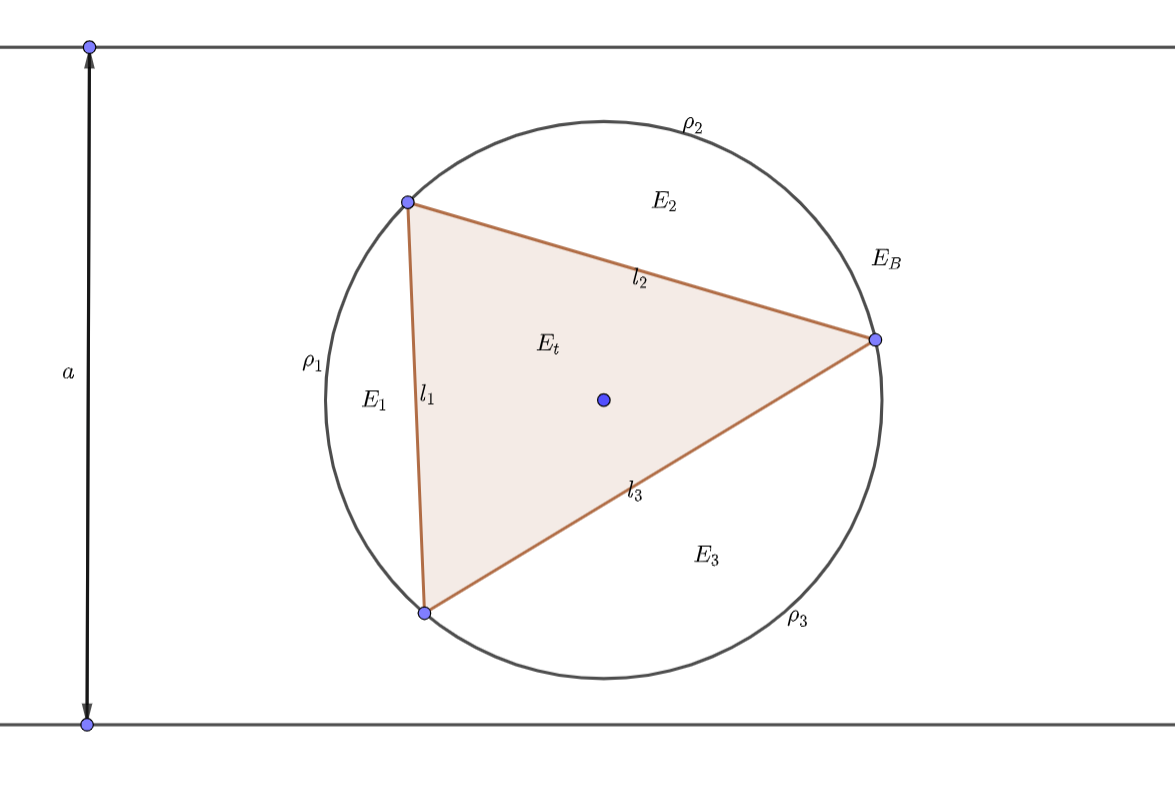
\includegraphics[width=0.8\textwidth]{figure.png}
}
% 表格模板
\renewcommand\arraystretch{0.8} % 设置表格高度为原来的0.8倍
\begin{table}[!htbp] % table标准
    \centering % 表格居中
    \begin{tabular}{p{1cm}<{\centering}p{1cm}<{\centering}p{3cm}<{\centering}p{5cm}<{\centering}} % 设置表格宽度
    %\begin{tabular}{cccc}
        \toprule
        $x_i$ & $f[x_1]$ & $f[x_i,x_{i+1}]$ & $f[x_i,x_{i+1},x_{i+2}]$ \\
        \midrule
        $x_0$ & $f(x_0)$ &                  &                          \\
        $x_0$ & $f(x_0)$ & $f'(x_0)$        &                          \\
        $x_0$ & $f(x_1)$ & $\frac{f(x_1)-f(x_0)}{x_1-x_0}$ & $\frac{f(x_1)-f(x_0)}{(x_1-x_0)^2}-\frac{f'(x_0)}{x_1-x_0}$\\
        \bottomrule
    \end{tabular}
\end{table}

\def\Log{\text{Log}} % 一个简单的宏定义
$\Log$ % 调用方法
\fi

\end{document}